\documentclass[dvipsnames, 10pt, compress]{beamer}

\usetheme{metropolis}
\usepackage{appendixnumberbeamer}

\usepackage{tikz-dependency}
\usepackage{caption}
%\usepackage{booktabs}
%\usepackage{tabularx}
\usepackage{alltt}
\usepackage[scale=2]{ccicons}

\usepackage{tikz-qtree}
\usepackage[linguistics]{forest}
\usepackage{pgfplots}
\usepgfplotslibrary{dateplot}

\usepackage{xspace}
\usepgflibrary{shapes.arrows}
\newcommand{\themename}{\textbf{\textsc{metropolis}}\xspace}


% commands from the paper
\newfontfamily\gtfont[Scale=1.1,Letters=SmallCaps]{Linux Libertine O}
\newcommand{\udtag}[1]{{\ll \textsc{#1}}}
\newcommand{\gtlabel}[1]{{\gtfont #1}}
\newcommand{\udlabel}[1]{{\tt #1}}
\newfontfamily\udfont[Scale=0.9,Letters=SmallCaps]{Linux Libertine O}
\newcommand{\utag}[1]{{\udfont#1}}
\newcommand{\ufeat}[1]{{\udfont#1}}
\newcommand{\tgl}[1]{{\em #1}}
\setmonofont[Scale=MatchLowercase]{DejaVu Sans Mono}

% commands from the paper

\newcommand*{\mystrut}{\rule[0.2\baselineskip]{0pt}{0.2\baselineskip}}
\newcommand{\redbox}[1]{\fcolorbox{red}{white}{\mystrut #1}}
\newcommand{\bluebox}[1]{\fcolorbox{ProcessBlue}{white}{\mystrut #1}}
\newcommand{\greenbox}[1]{\fcolorbox{YellowGreen}{white}{\mystrut #1}}
\newcommand{\redfillbox}[1]{\colorbox{red}{\textcolor{white}{{\bf #1}}}}
\newcommand{\bluefillbox}[1]{\colorbox{ProcessBlue}{\textcolor{white}{{\bf #1}}}}
\newcommand{\greenfillbox}[1]{\colorbox{YellowGreen}{\textcolor{white}{{\bf #1}}}}
%\newcommand*{\mybox}[1]{\framebox{\strut #1}}

\newcommand{\myarrow}[1][-45]{%
  \mathrel{%
    \text{$
     \begin{tikzpicture}[baseline = -0.5ex]
       \node[inner sep=0pt,outer sep=0pt,rotate = #1] (a) at (0,0)  {$\xrightarrow{}$};
    \end{tikzpicture}
    $}%
  }%
}%




\title{Class 11: Anaphora and co-reference resolution}
\date{}
\begin{document}
\tikzstyle{side arrow} = [draw=black!75, very thick, double arrow, minimum height=5.0cm, shape border rotate =#1, fill=gray!10]

\maketitle

\begin{frame}{Things and naming things}



\end{frame}

\begin{frame}{What is co-reference resolution?}

\begin{onlyenv}<1>
THE prime minister has fired secretary of state Priti Patel while telling 
her she wishes with all her heart it was the other way around. 

May confessed to Patel that although having secret meetings with the Israelis 
was a sackable offence, it paled in comparison to her own dire 
performance but “sadly nobody’s willing to pull the trigger.” 

Patel said: “It was so awkward. She said ‘You don’t know how often I’ve dreamt of 
sitting on your side of the desk, finally being summarily dismissed for 
my gross incompetence.’ 
\end{onlyenv}

\begin{onlyenv}<2>
\begin{center}
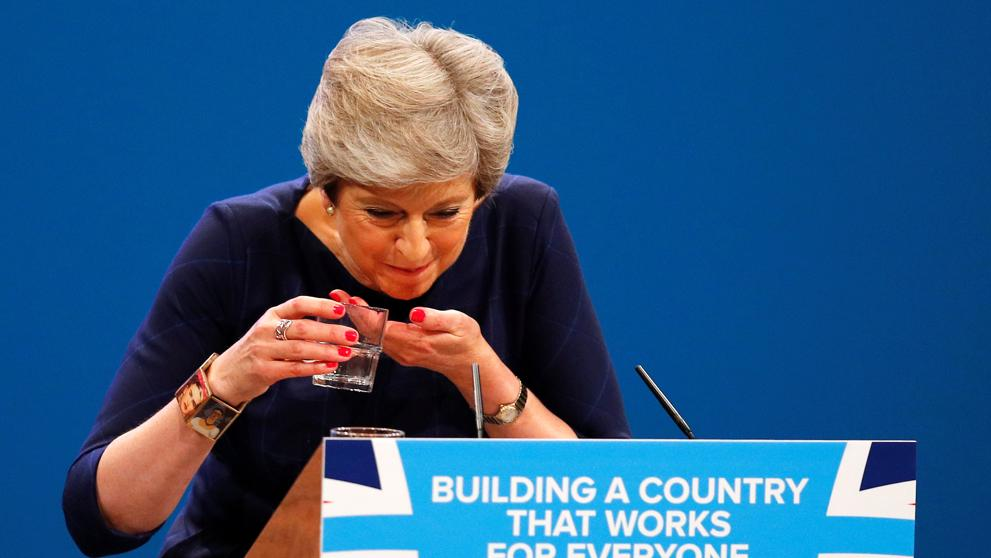
\includegraphics[width=0.4\textwidth]{graphics/theresa-may.jpg}
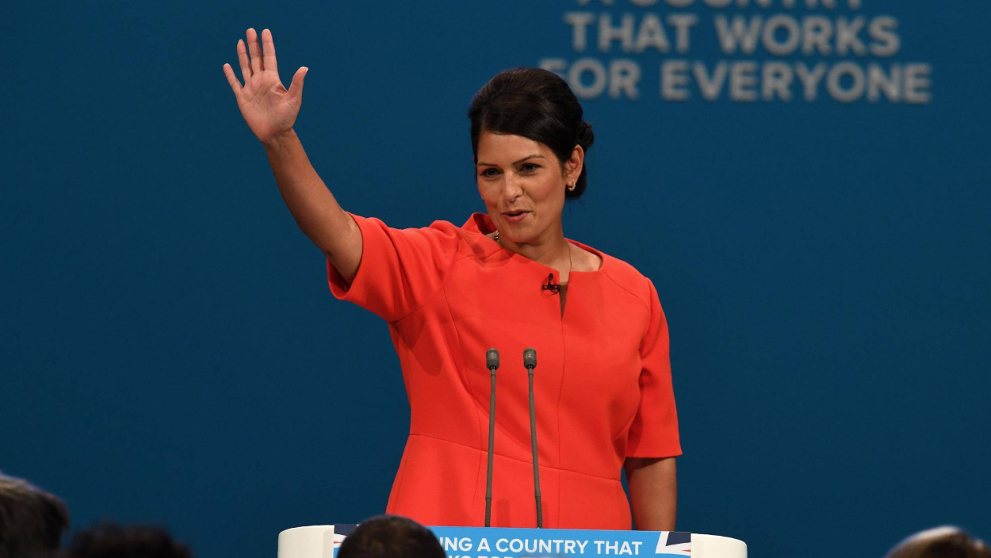
\includegraphics[width=0.4\textwidth]{graphics/priti-patel.jpg}
\end{center}
THE prime minister has fired secretary of state Priti Patel while telling 
her she wishes with all her heart it was the other way around. 

May confessed to Patel that although having secret meetings with the Israelis 
was a sackable offence, it paled in comparison to her own dire 
performance but “sadly nobody’s willing to pull the trigger.” 

Patel said: “It was so awkward. She said ‘You don’t know how often I’ve dreamt of 
sitting on your side of the desk, finally being summarily dismissed for 
my gross incompetence.’ 
\end{onlyenv}


\begin{onlyenv}<3>
\begin{center}
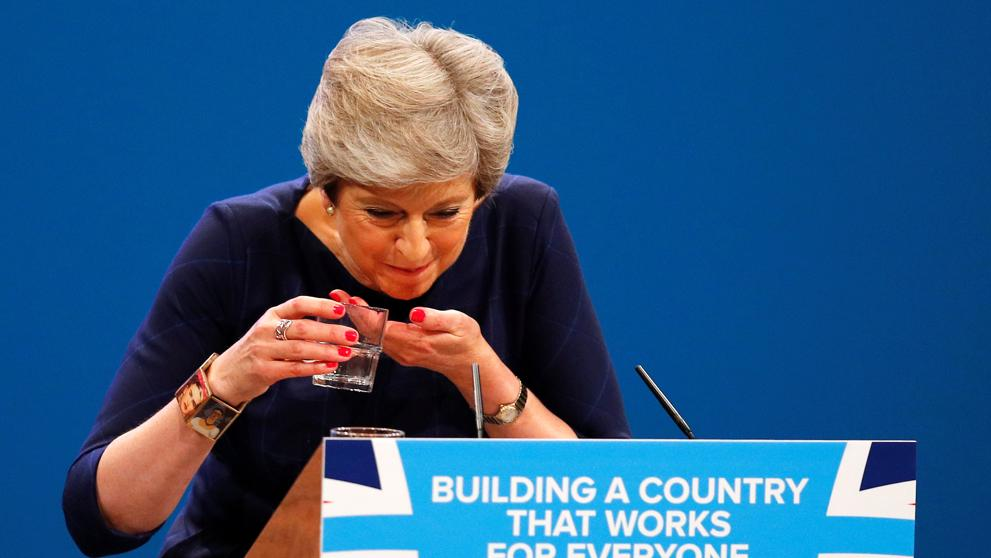
\includegraphics[width=0.4\textwidth]{graphics/theresa-may.jpg}
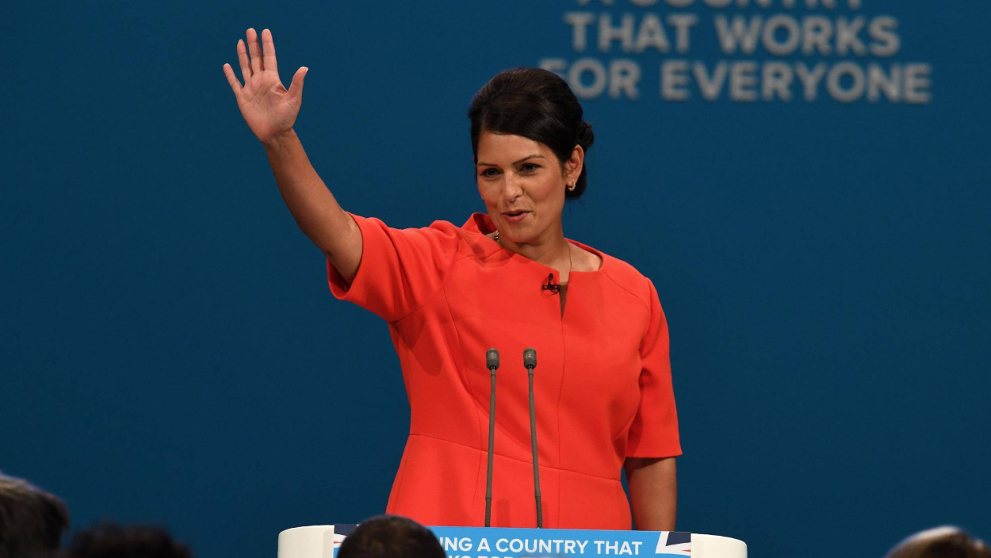
\includegraphics[width=0.4\textwidth]{graphics/priti-patel.jpg}
\end{center}
\colorbox{ProcessBlue}{\textcolor{white}{{\bf THE prime minister}}} has fired secretary of state Priti Patel while telling 
her \colorbox{ProcessBlue}{\textcolor{white}{{\bf she}}} wishes with all \bluebox{her} heart it was the other way around. 

\colorbox{ProcessBlue}{\textcolor{white}{{\bf May}}} confessed to Patel that although having secret meetings with the Israelis 
was a sackable offence, it paled in comparison to \bluebox{her} own dire 
performance but “sadly nobody’s willing to pull the trigger.” 

Patel said: “It was so awkward. \colorbox{ProcessBlue}{\textcolor{white}{{\bf She}}} said ‘You don’t know how often \colorbox{ProcessBlue}{\textcolor{white}{{\bf I}}}’ve dreamt of 
sitting on your side of the desk, finally being summarily dismissed for 
\bluebox{my} gross incompetence.’ 
\end{onlyenv}

\begin{onlyenv}<4>
\begin{center}
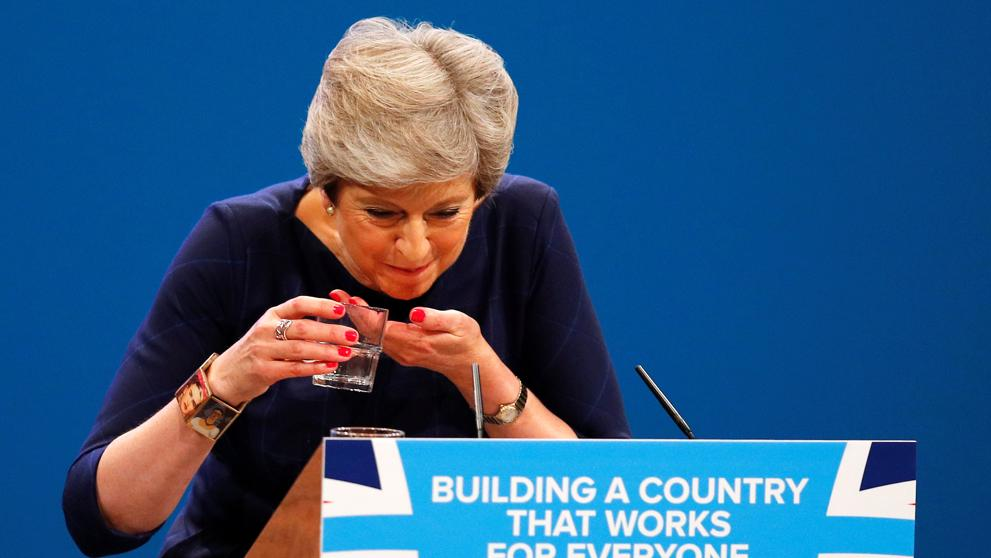
\includegraphics[width=0.4\textwidth]{graphics/theresa-may.jpg}
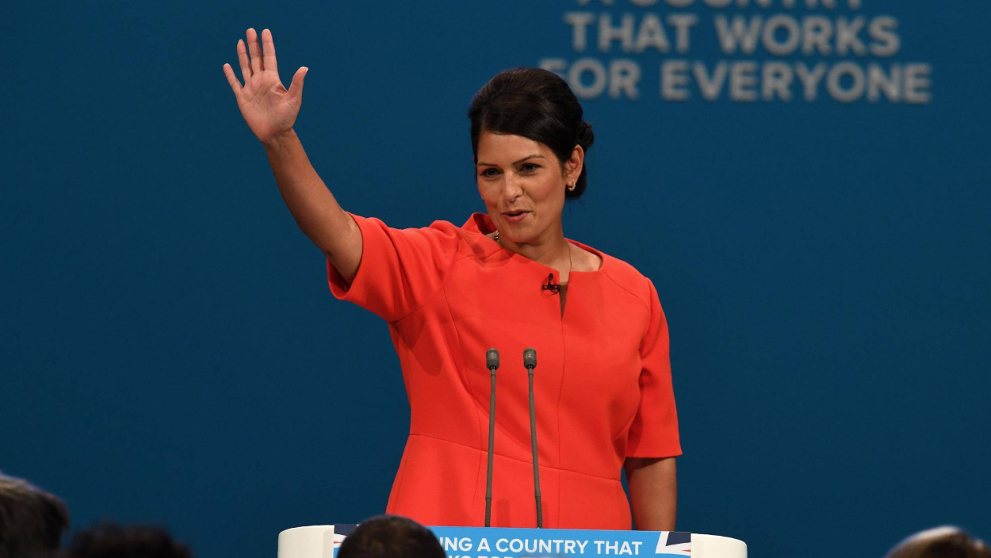
\includegraphics[width=0.4\textwidth]{graphics/priti-patel.jpg}
\end{center}
THE prime minister has fired \colorbox{red}{\textcolor{white}{{\bf secretary of state}}} \colorbox{red}{\textcolor{white}{{\bf Priti Patel}}} while telling 
\colorbox{red}{\textcolor{white}{{\bf her}}} she wishes with all her heart it was the other way around. 

May confessed to \colorbox{red}{\textcolor{white}{{\bf Patel}}} that although having secret meetings with the Israelis 
was a sackable offence, it paled in comparison to her own dire 
performance but “sadly nobody’s willing to pull the trigger.” 

\redfillbox{Patel} said: “It was so awkward. She said ‘\colorbox{red}{\textcolor{white}{{\bf You}}} don’t know how often I’ve dreamt of 
sitting on \redbox{your} side of the desk, finally being summarily dismissed for 
my gross incompetence.’ 
\end{onlyenv}

\begin{onlyenv}<5>
\begin{center}
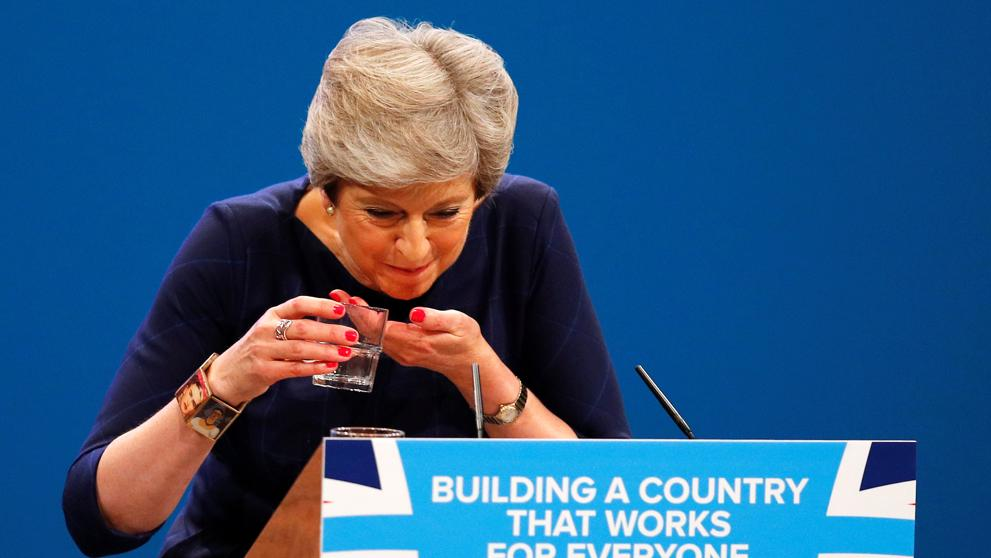
\includegraphics[width=0.4\textwidth]{graphics/theresa-may.jpg}
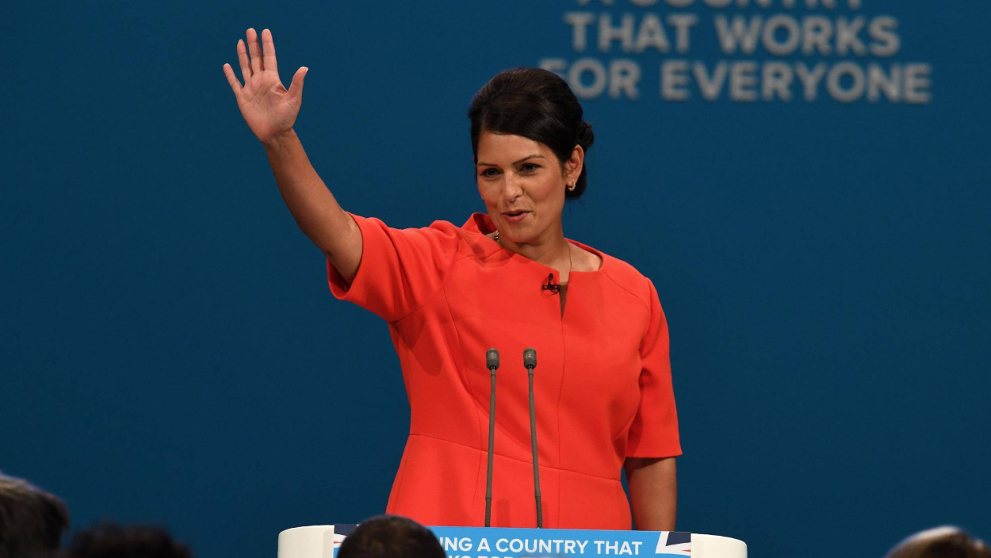
\includegraphics[width=0.4\textwidth]{graphics/priti-patel.jpg}
\end{center}
\bluefillbox{THE prime minister} has fired \colorbox{red}{\textcolor{white}{{\bf secretary of state}}} \colorbox{red}{\textcolor{white}{{\bf Priti Patel}}} while telling 
\colorbox{red}{\textcolor{white}{{\bf her}}} \bluefillbox{she} wishes with all \bluebox{her} heart it was the other way around. 

\bluefillbox{May} confessed to \colorbox{red}{\textcolor{white}{{\bf Patel}}} that although having secret meetings with the Israelis 
was a sackable offence, it paled in comparison to \bluebox{her} own dire 
performance but “sadly nobody’s willing to pull the trigger.” 

\redfillbox{Patel} said: “It was so awkward. \bluefillbox{She} said ‘\colorbox{red}{\textcolor{white}{{\bf You}}} don’t know how often \bluefillbox{I}’ve dreamt of 
sitting on \redbox{your} side of the desk, finally being summarily dismissed for 
\bluebox{my} gross incompetence.’ 
\end{onlyenv}


\end{frame}

\begin{frame}{Noun phrases and reference}

\fbox{\parbox{\textwidth}{
\begin{itemize}
\item NPs usually refer to entities in the world
\item NPs may co-refer, meaning they refer to the same entity
\item They may also be nested or discontinuous % Peter came there with Masha. They...
\end{itemize}}}

Однажды \bluefillbox{Пушкин} написал письмо \redfillbox{Рабиндранату Тагору}. 
«\redfillbox{Дорогой далекий друг}, — писал \bluefillbox{он}, — \bluefillbox{я} \redfillbox{Вас} не знаю, и \redfillbox{Вы} \bluefillbox{меня} не знаете.
Очень хотелось бы познакомиться. Всего хорошего. \bluefillbox{Саша}».
Когда письмо принесли, \redfillbox{Тагор} предавался самосозерцанию. 
Так погрузился, хоть режь \redfillbox{его}. 
\greenfillbox{\redbox{\textcolor{black}{Его}} жена} толкала, толкала, письмо подсовывала — не видит. 
\redfillbox{Он}, правда, по-русски читать не умел. Так и не познакомились.



\end{frame}

\begin{frame}{Kinds of reference}

\begin{columns}

\column{0.2\textwidth}

\begin{tikzpicture}[overlay]
\node[draw] at (1,3.0) {Easier};
\node[draw] at (1,-3.0) {Harder};
\node at (1,0) [side arrow=90] {\rotatebox{90}{~}};
\end{tikzpicture}


\column{0.8\textwidth}

Interesting linguistics 
~\\
~\\

\begin{tabular}{ll}

\textbf{Bound variables} & She hurt \emph{herself} \\
                         & Я имею \emph{свой} баян \\
% Bound variables [She hurt herself]

%% Only possible analysis is coreferent with the subject

% Free variables [She saw her pay increase] -- [Она видела ее/свой]
~ & ~ \\
\textbf{Free variables} & Maša read \emph{her} book \\
                        & \emph{Ей} очень нравилась. \\

%% Might be coreferent with the subject or not

% Referring expressions 
~ & ~ \\

\textbf{Referring expressions} & Carles Puigdemont \\
                               & the Catalan president \\
                               & Puigdemont \\ 
                               & Puchi \\ 
                               & president of Catalonia \\
                               & President Puigdemont \\
%% 
\end{tabular}

More frequent

\end{columns}

\end{frame}

\begin{frame}{Coreference, anaphora, cataphora}

\begin{itemize}
  \item  \textbf{Coreference} 
  \begin{itemize}  
    \item Two \emph{mentions} (NPs) refer to the same entity 
    \item May be identical or completely different
  \end{itemize}
  \item \textbf{Anaphora, Cataphora} 
  \begin{itemize}
    \item Interpretation is in some way dependent on an antecedent
    \item Traditionally the antecedent came first, but not always the case.
  \end{itemize}
\end{itemize}

\end{frame}


\begin{frame}{Cataphora}

%From the corner of the divan of Persian saddlebags on which he was lying, smoking, as was his custom, innumerable cigarettes, Lord Henry Wotton could just catch the gleam of the honey-sweet and honey-coloured blossoms of a laburnum, whose tremulous branches seemed hardly able to bear the burden of a beauty so flame-like as theirs;...

% С покрытого персидскими чепраками дивана, на котором лежал лорд Генри Уоттон, куря, как всегда, одну за другой бесчисленные папиросы, был виден только куст ракитника -- его золотые и душистые, как мед, цветы жарко пылали на солнце, а трепещущие ветви, казалось, едва выдерживали тяжесть этого сверкающего великолепия \ldots


(Oscar Wilde -- The Picture of Dorian Grey)
%
%<padre_angolano> spectie: "Еще раз сверившись с бумажкой, на которой он все-таки вопреки советам Васи записал адрес, Пафнутьев направился к стоянке такси"
%<padre_angolano> spectie: "Внимательно вглядываясь в несущуюся под ногами тропинку, на которую он обычно садился, Митя широко раскрыл крылья, повернул их навстречу бьющему в лицо воздуху"

\end{frame}

\begin{frame}{Other types of anaphora}

\begin{itemize}
  \item Bridging Anaphora: 
  \item "Other" Anaphora: 
  \item Non-NP Anaphora (e.g. events, propositions)

\end{itemize}

\end{frame}


\begin{frame}{Anaphora vs. coreference}

\begin{itemize}
  \item Not all anaphoric relations are coreferential, e.g. bridging anaphora
  \item Multiple identical NP matches are often coreferential but not anaphoric
\end{itemize}

\end{frame}

% example

\begin{frame}{Two different things}


\begin{tikzpicture}[overlay]
\node at (7,3.0) {\textbf{Anaphora resolution}};
\node at (1,2.0) {\textbf{Text}};
\node at (1,0.5) {\textbf{World}};
\node[draw] at (5,2.0) {~};
\node[draw] at (9,2.0) {~};
\node[draw] at (5,0.5) {~};
%\node[draw=black!75, thin, double arrow, minimum height=3.0cm, fill=gray!10] at (7,2.0) {~~~~} ;
%\node[draw=black!75, thin, double arrow, shape border rotate=90, minimum height=1.0cm, fill=gray!10] at (5,1.0) {~~~~} ;
\draw[<-,line width=1pt] (5.5,2.0) to (8.5,2.0);
\draw[->,line width=1pt] (5.0,1.6) to (5.0,0.8);
\end{tikzpicture}

~\\

\begin{tikzpicture}[overlay]
\node at (7,0.5) {\textbf{Co-reference resolution}};
\node at (1,-0.5) {\textbf{Text}};
\node at (1,-2.0) {\textbf{World}};
\node[draw] at (5,-0.5) {~};
\node[draw] at (9,-0.5) {~};
\node[draw] at (7,-2.0) {~};
\draw[->,line width=1pt] (5.5,-0.75) to (6.8,-1.8);
\draw[->,line width=1pt] (8.5,-0.75) to (7.2,-1.8);
\end{tikzpicture}

\end{frame}

\begin{frame}{Applications}

\textbf{Machine translation:}
\begin{itemize}
  \item Translating pronouns like \emph{себя} --- myself, yourself, herself, \ldots
  \item Translating from languages with no gender distinction in pronouns \emph{hän} --- \emph{он, она}
\end{itemize}

\textbf{Text summarisation:}
\begin{itemize}
  \item ~[Maša]$_i$ read [Wikipedia]$_j$ with unbridled enthusiasm. [She]$_i$ spent so long reading [it]$_j$ that [she]$_i$ 
     forget about her homework. 
     \begin{itemize}
        \item[$\rightarrow$] Maša read Wikipedia and forgot about her homework.
     \end{itemize}
\end{itemize}
\textbf{Information extraction:}
\begin{itemize}
  \item What did Maša do ? 
  \begin{itemize}
    \item read Wikipedia
    \item forgot about her homework
  \end{itemize}
\end{itemize}

\end{frame}

% ALGORITHMS

\section{Pronominal anaphora resolution}

%\begin{frame}


%\end{frame}

\begin{frame}{Hobbs' (1978) algorithm/1}

\begin{itemize}
  \item Simple syntax-based algorithm for 3rd person anaphoric pronouns
  \item Requires:
  \begin{itemize}
     \item Constituency parser
     \item Gender and number `checker'
     \begin{itemize}
        \item Parsers for English rarely include gender information for nouns
     \end{itemize}
  \end{itemize}
  \item Searches current and preceding sentences in a breadth-first, left-to-right
     manner, stops when it finds a matching NP
\end{itemize}

\end{frame}

\begin{frame}{Hobbs' (1978) algorithm/2}

\begin{itemize}
  \item Right to left search in current sentence 
  \item If not valid antecedent fine, try previous sentence
  \begin{itemize}
    \item Left to right breadth-first search
  \end{itemize}
 
\end{itemize}

\end{frame}

\begin{frame}{Hobbs' (1978) algorithm/3}

\begin{onlyenv}<1>

\includegraphics[width=\textwidth]{graphics/drone-training-2x.png}
\end{onlyenv}
\begin{onlyenv}<2>

\includegraphics[width=\textwidth]{graphics/drone-training-2x-2.png}
\end{onlyenv}


\end{frame}

\begin{frame}{Hobbs' (1978) algorithm/4}
%My drone keeps flying into the wrong rooms.
%Do you have anything to discourage it?

\begin{columns}

\column{0.6\textwidth}
%\begin{tikzpicture}
%\Tree [.S [.DP My [.NP drone]] [.VP [.V keeps] [.Comp flying [.PP into [.DP the [.NP [.AP [.A wrong] [.N rooms]]]]]]]]
%\end{tikzpicture}
\scalebox{0.8}{
\begin{forest}
[S$_1$ [NP$_1$ [My drone]] [VP [V [keeps flying]] [PP [into] [NP$_2$ [the wrong rooms]]]]]
%[S 
%  [NP [My drone] ]
%  [VP [keeps 
%        flying [PP [into] [the [NP [wrong] [rooms]]]]]]
%]
\end{forest}
}
~\\
~\\
\begin{itemize}
   \item Start search in NP$_5$ in S$_2$
   \item Reject NP$_4$, no intervening NP
   \item Reject NP$_3$, feature mismatch
   \item Move to S$_1$
   \item Accept NP$_1$
\end{itemize}
\column{0.4\textwidth}
\scalebox{0.8}{
\begin{forest}
[S$_2$ [Do] [S$_3$ [NP$_3$ [You]] [VP [have] [SC [NP$_4$ [anything]] [Inf [to] [VP [discourage] [NP$_5$ [it]]]]]]]]
\end{forest}
}
\end{columns}

\end{frame}

\begin{frame}{Log-linear model/1} % General idea

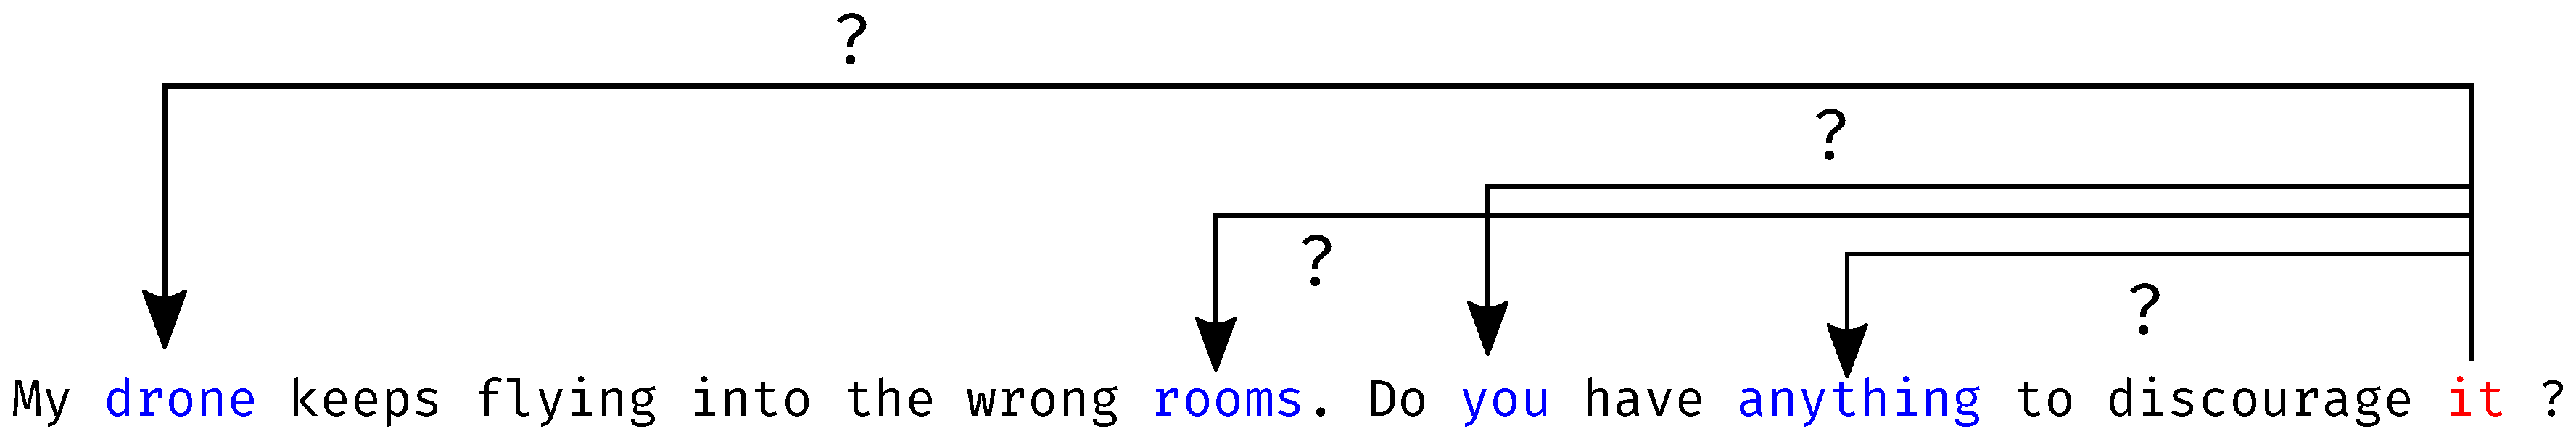
\includegraphics[width=\textwidth]{graphics/classifier-coref-2.eps}

\begin{itemize}
  \item Supervised machine learning approach
  \item Requires corpus where each pronoun has been linked with its antecedent
\end{itemize}

\begin{itemize}
  \item Extract positive and negative examples
  \item Train binary classifier 
  \begin{itemize}
     \item True: is co-referent
     \item False: is not co-referent
  \end{itemize}
\end{itemize}

\end{frame}

\begin{frame}{Log-linear model/2} % Positive and negative examples
%My drone keeps flying into the wrong rooms.
%Do you have anything to discourage it?

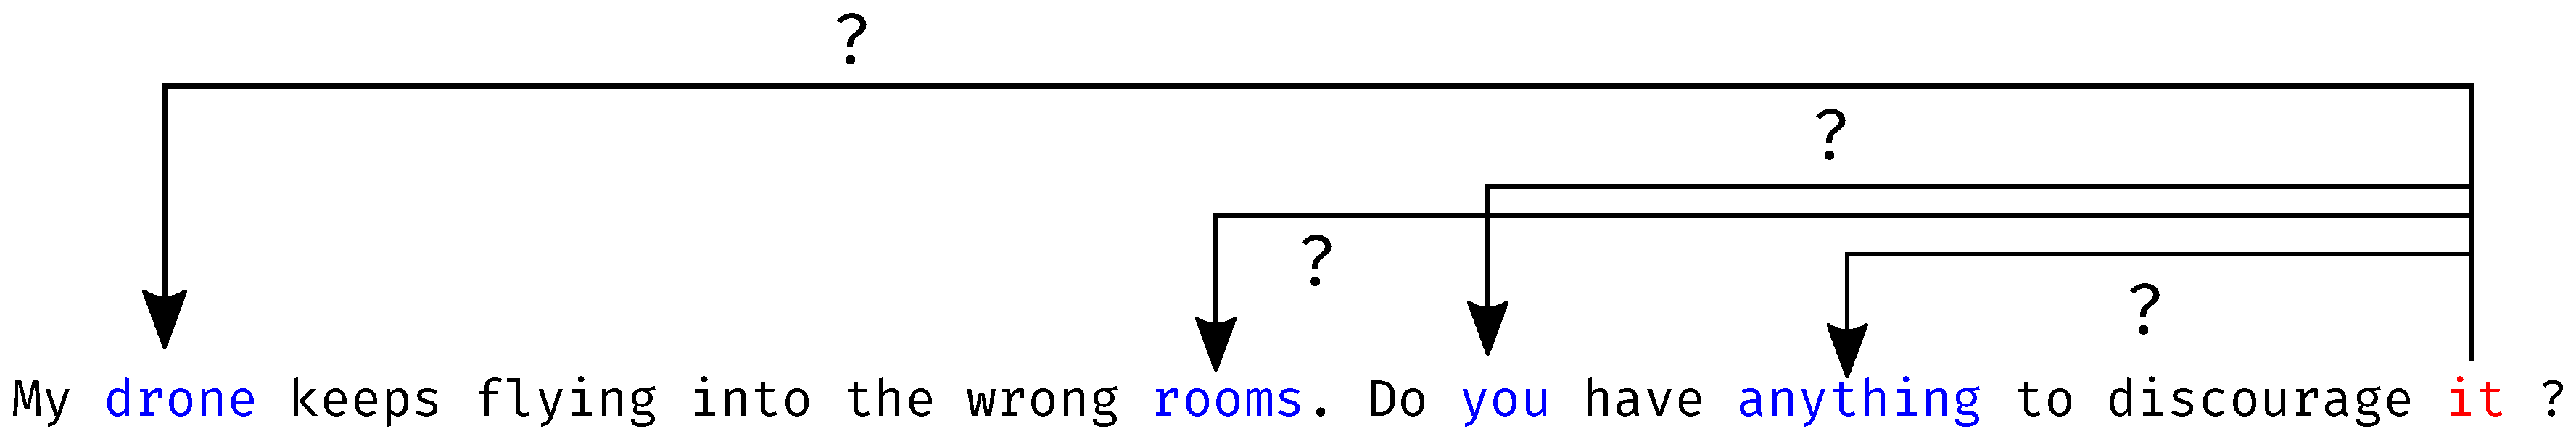
\includegraphics[width=\textwidth]{graphics/classifier-coref-2.eps}

Positive example:
\begin{itemize}
 \item (it, my drone)
\end{itemize}

Negative examples:
\begin{itemize}
 \item (it, anything)
 \item (it, you)
 \item (it, the wrong rooms)
\end{itemize}

\end{frame}

\begin{frame}{Log-linear model/3} % Features

\begin{itemize}
  \item \textbf{strict gender} [true, false]
  \item \textbf{compatible gender} [true, false]
  \item \textbf{strict number} [true, false]
  \item \textbf{compatible number} [true, false]
  \item \textbf{sentence distance} [0, 1, 2, \ldots]
  \item \textbf{Hobbs distance} [0, 1, 2, \ldots] 
  \item \textbf{linguistic form} [proper, def, indef, pronoun]
\end{itemize}

Can you think of some other useful features ? 

\end{frame}

\begin{frame}{Log-linear model/4}

\begin{itemize}
 \item \textbf{Recency:} More recently mentioned entities are more likely to be referred to 
 \item \textbf{Grammatical Role:} Entities in the subject position is 
more likely to be referred to than entities in the object 
position 
 \item \textbf{Parallelism:}
 \item \textbf{Verb Semantics:} Certain verbs seem to bias whether 
the subsequent pronouns should be referring to their 
subjects or objects 
 \item \textbf{Selectional Restrictions:} Restrictions because of 
semantics 
\end{itemize}

\end{frame}

\begin{frame}{Log-linear model/5} % Applying the model

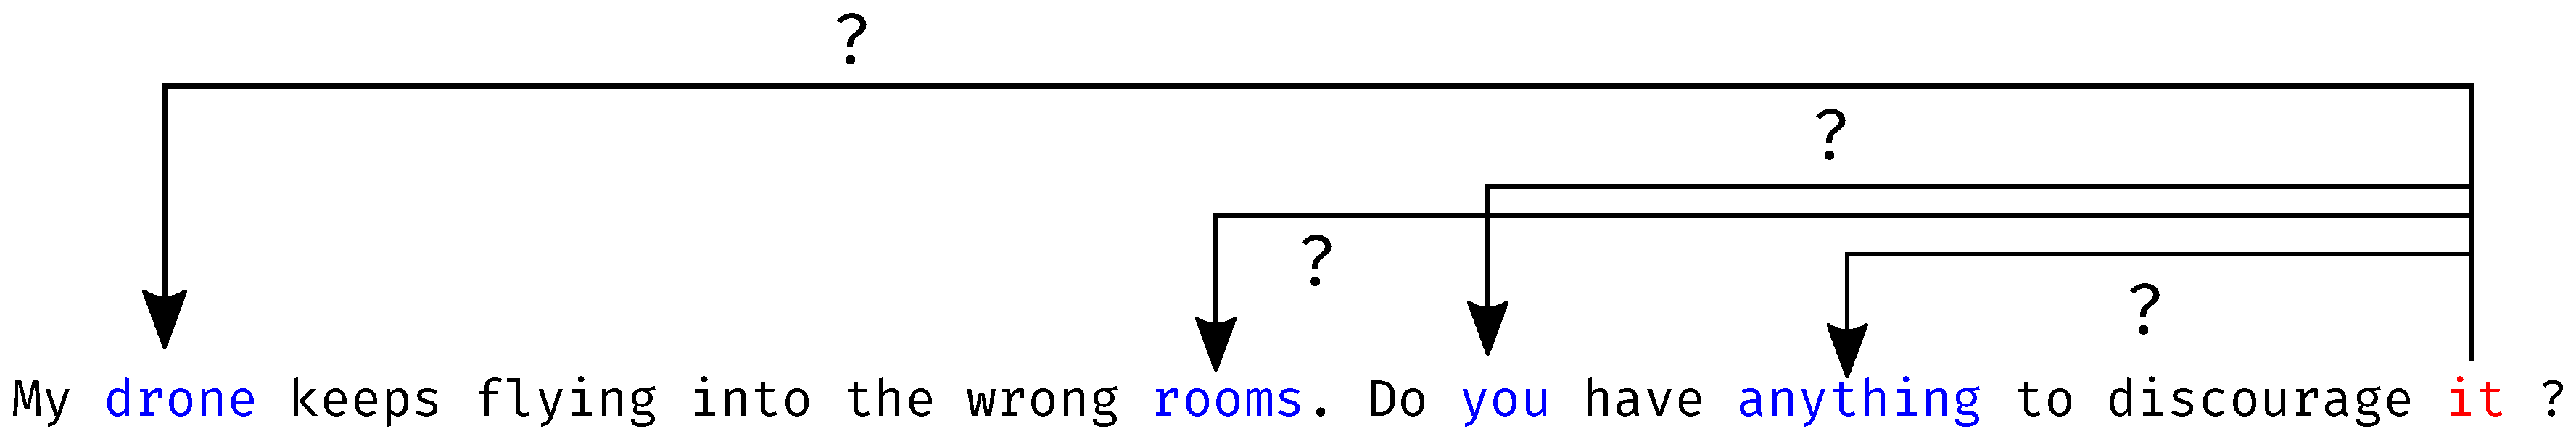
\includegraphics[width=\textwidth]{graphics/classifier-coref-2.eps}

\begin{itemize}
  \item For each pronoun,
  \begin{itemize}
     \item For each NP we have seen so far,
     \begin{itemize}
       \item Classify if NP is an antecedent of the pronoun
     \end{itemize}
  \end{itemize}
\end{itemize}


\end{frame}

\section{Co-reference resolution}


\begin{frame}


\end{frame}


\begin{frame}{Reference models}

% chains , entity-mention , 

Однажды \bluefillbox{Пушкин} написал письмо \redfillbox{Рабиндранату Тагору}. 
«\redfillbox{Дорогой далекий друг}, — писал \bluefillbox{он}, — \bluefillbox{я} \redfillbox{Вас} не знаю, и \redfillbox{Вы} \bluefillbox{меня} не знаете.
Очень хотелось бы познакомиться. Всего хорошего. \bluefillbox{Саша}».
Когда письмо принесли, \redfillbox{Тагор} предавался самосозерцанию. 
Так погрузился, хоть режь \redfillbox{его}. 
\greenfillbox{Его жена} толкала, толкала, письмо подсовывала — не видит. 
\redfillbox{Он}, правда, по-русски читать не умел. Так и не познакомились.

\begin{tabular}{l}
{ Пушкин, он$_1$, я$_1$, меня$_1$ } \\ 
{ Рабиндранату Тагору, Дорогой далекий друг, Вас$_1$, Вы$_1$, Тагор, его$_1$, Он} \\
\end{tabular}

\end{frame}

\begin{frame}{General algorithm}

\end{frame}


\begin{frame}{Additional features}

\end{frame}


\begin{frame}{Rule-based models/1} % xrenner

Input is a sequence of dependency trees representing the document.

Constraint-based, rules like:

$C = <ANA,  ANT, DIST, PROP>$

\begin{itemize}
  \item ANA, ANT = constraints on the anaphor and antecedent
  \item DIR = direction (e.g. forward, backwards)
  \item DIST = how far to look (in sentences)
  \item PROP = should features (e.g. gender) be propagated?
\end{itemize}

\end{frame}

\begin{frame}{Rule-based models/2} % xrenner

Example rules:

\begin{itemize}
  \item Mark full-text matches as coreferent
  \item Two 1st person pronouns in the same quoted speech corefer
  \item A surname matching a previous firstname + surname corefers
\end{itemize}

\end{frame}


\section{Evaluation}

% EVALUATION

\begin{frame}{Model-Theoretic coreference scoring/1}

Used in the MUC series of shared tasks

Requires:
\begin{itemize}
  \item A KEY (the gold standard)
  \item A RESPONSE (system output)
\end{itemize} 

\end{frame}

\begin{frame}{Model-Theoretic coreference scoring/2}

Given that A,B,C and D are part of a coreference 
chain in the KEY, treat as equivalent the two 
responses: 
\begin{center}

\includegraphics[width=0.8\textwidth]{graphics/coref-eval-1.png}
\end{center}

And as superior to: 
\begin{center}

\includegraphics[width=0.8\textwidth]{graphics/coref-eval-2.png}
\end{center}
\end{frame}

\begin{frame}{Model-Theoretic coreference scoring/3}

\begin{center}
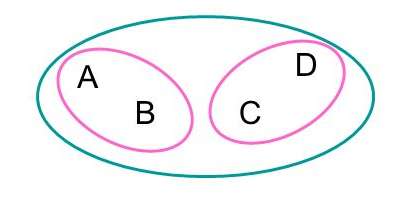
\includegraphics[width=0.5\textwidth]{graphics/coref-scoring-1.png}
\end{center}

\begin{itemize}
  \item KEY: [A, B, C, D]
  \item RESPONSE: [A, B] [C, D]
\end{itemize}

\begin{itemize}
  \item Recall = $\frac{4 - 2}{3} = 0.66$
  \item Precision = $\frac{4 - 1}{4 - 1} = 1.0$
  \item F-score = $\frac{2 . \frac{2}{3} * 1}{\frac{2}{3} . 1} = 0.79$
\end{itemize}
\end{frame}

\begin{frame}{Other metrics}

\begin{itemize}
   \item B$^3$ scoring
    \item CEAF
\end{itemize}

\end{frame}

\section{Tools and resources}

\begin{frame}{Stanford CoreNLP}

\begin{center}

\includegraphics[width=\textwidth]{graphics/Xi-Jinping.png} \\
\url{https://stanfordnlp.github.io/CoreNLP/index.html}
\end{center}

\begin{itemize}
 \item includes coreference for English + Chinese
 \item rule-based, statistical and neural models
 \item based on Java
 \item very ``heavy'' ($>$ 1G for code + model)
\end{itemize}

\end{frame}

\begin{frame}{xrenner}

\begin{center}
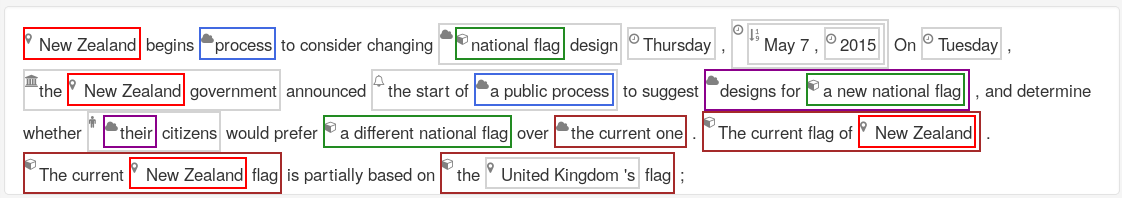
\includegraphics[width=\textwidth]{graphics/xrenner.png} \\
   e\textbf{X}ternally configurable \textbf{RE}ference and \textbf{N}on \textbf{N}amed \textbf{E}ntity \textbf{R}ecogniser \\
\url{https://github.com/amir-zeldes/xrenner}

\end{center}

\begin{itemize}
  \item based on Python
  \item Rule-based (constraints)
  \item Functioning model for English
  \item (relatively) small footprint ($<$ 100M)
\end{itemize}

% model for English

\end{frame}

\begin{frame}{RuCor}

\begin{center}
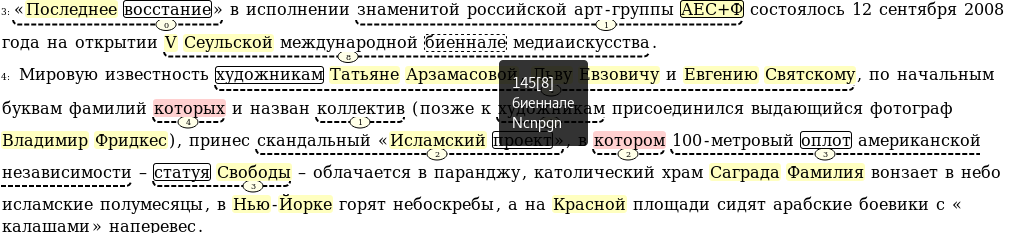
\includegraphics[width=\textwidth]{graphics/rucoref-pic.png} \\
\url{http://ant1.compling.net/res03/ant1.php}
\end{center}


\begin{itemize}
  \item Corpus of Russian annotated for co-reference
  \item 156,636 tokens

\end{itemize}

\end{frame}

% ruCoRef http://rucoref.maimbava.net/
% OntoNotes

\section{Shared tasks}
% SHARED TASK(S)

\begin{frame}{Message Understanding Conference (MUC)}

%One of the first evaluation events for the tasks under discussion took place within
%the Message Understanding Conferences (MUCs). The following definition for the
%coreference relations was suggested: “The coreference ‘layer’ links together multiple
%expressions designating a given entity”. Only links between noun phrases were con-
%sidered. The main criteria for the task definition were the good interannotator agree-
%ment, the simplicity and speed of text annotation, the objective to create a corpus for
%independent research of coreference. The MUC project is the best-known example
%of coreference annotation, on which much subsequent work is based. The various
%systems results on the test sets from MUC-6 (1995) and MUC-7 (1998) coreference
%corpora are widely discussed in the literature (c.f. [Mitkov 1999], [Van Deemter, K., &
%Kibble, R. 2000] and others). The main principle for data annotation was the referen-
%tial NP identity. We followed the basic MUC data annotation principles

\end{frame}

\begin{frame}{SemEval 2010}

%The SemEval-2010 task is of special interest for us in the following respect:
%it is the task task on Coreference Resolution in Multiple Languages (six languages
%such as Catalan, Dutch, English, German, Italian and Spanish). Besides the well-stud-
%ied languages, the under-resourced languages took part in the anaphora resolution
%procedure. Some of the participants used small training and testing data sets (e.g.
%80 texts for Italian as a training set and 46 texts as a test set). The other issue of inter-
%est is that four different metrics were used in evaluation. The corpora were annotated
%with morphological, syntactic and partial semantic tags. One of the aims of the event
%was to learn out what was the impact of different levels of linguistic information.



\end{frame}

\begin{frame}{RuEval-2014}

Two tracks:
\begin{itemize}
  \item Pronominal anaphora resolution (8 teams)
  \begin{itemize}
     \item personal, possessive, relative and reflexive pronouns
     \item antecedent should be in the gold-standard coreference chain
  \end{itemize}
  \item Co-reference resolution (3 teams)
\end{itemize}



\end{frame}

\section{Practical}

\begin{frame}{Practical}

For the practical, select a short paragraph or document and write some coreference rules 
using Xrenner.

Further instructions:

\url{https://ftyers.github.io/028-komp-ling/classes/11.html}

\end{frame}

\end{document}
